\section{Functionality}

\subsection{Object Storage and data preprocessing}
The current status of our project involves the establishment of a rudimentary
data lake infrastructure, meticulously crafted using robust and efficient
Raspberry Pi servers. This infrastructure serves as the bedrock upon which we
have meticulously implemented several essential features, akin to those
prevalent in established data lake systems.

Foremost among these features is the implementation of a versatile gateway,
meticulously designed to seamlessly ingest data from an array of incoming
sources, ranging from radars to sensors. This gateway boasts compatibility with
the Amazon Web Service S3-compatible API, rendering it universally accessible to
clients and libraries engineered to interface with such protocols. Its
compatibility with this widely adopted standard ensures that our gateway can
seamlessly integrate with a plethora of external sources, thus enhancing the
scalability and versatility of our infrastructure manifold.

Moreover, a robust platform for Data Orchestration has been deployed, with
Apache Airflow serves as its cornerstone. This strategic implementation not
only streamlines the current data management processes but also lays a solid
foundation for the future scalability and expansion of our system. By
orchestrating the scheduling, monitoring, and reporting of all data flows within
the ecosystem, Airflow ensures the seamless integration of new tenants and
providers, thereby safeguarding the integrity and efficiency of our data
management operations.

In addition to these pivotal components, our team has diligently developed and
published PyTorch's native Data Loader to PyPI, a renowned package management
platform within the Python developer community. This initiative represents a
significant milestone in our endeavor to streamline data access and utilization
within our ecosystem. By providing researchers with a user-friendly library that
abstracts the complexities of low-level API interactions, we aim to
significantly reduce the learning curve associated with navigating our data lake
infrastructure. This strategic move not only enhances the accessibility of our
system but also fosters a conducive environment for innovation and collaboration
within the research community.

\subsection{Form Builder and advanced features}
The integration of the Form Builder as an add-on feature represents a strategic
enhancement tailored to cater to the specific needs of our discerning customer
base. Stemming from insights garnered during a comprehensive field trip to the
Nha Be radar station, our team identified an opportunity to streamline and
augment the operational workflow of operators tasked with responding to
hazardous weather conditions. In response to this pressing need, we proposed and
swiftly implemented the Form Builder feature, envisaging it as a pivotal tool in
facilitating the seamless completion of warning forms amidst adverse weather
events.

The preliminary implementation of the Building Form functionality marks an
auspicious milestone in the development trajectory of this feature. While it
remains in the nascent stages of development, we are optimistic about its
potential to address the operational inefficiencies and pain points encountered
by operators at the Nha Be radar station. By affording operators an intuitive
and user-friendly interface for form completion, we envisage a tangible
improvement in workflow efficiency and responsiveness, thereby bolstering the
station's capacity to effectively manage hazardous weather conditions.

Furthermore, beyond its immediate utility as a workflow enhancement tool, the
Form Builder feature holds promise as a source of valuable insights and data for
our team. Through the aggregation and analysis of hand-labeled data generated
during the form completion process, we anticipate gaining invaluable insights
into the operational dynamics and decision-making processes underpinning hazard
response scenarios. This rich repository of data not only informs iterative
improvements to the Form Builder feature but also serves as a springboard for
enhancing our understanding of user needs and preferences, thereby fostering a
culture of continuous improvement and innovation within our organization.

Looking ahead, we remain steadfast in our commitment to refining and optimizing
the Form Builder feature to meet the evolving needs and expectations of our
stakeholders. Through ongoing collaboration and feedback from end-users, we
endeavor to iteratively enhance the functionality and usability of this feature,
ensuring its seamless integration into the operational workflows of operators at
the Nha Be radar station. Moreover, we remain vigilant in our efforts to
leverage the insights gleaned from this initiative to inform future product
development endeavors, thereby solidifying our position as a trusted provider of
innovative solutions tailored to the unique challenges of weather hazard
response.

\section{Performance Evaluation}
Following the meticulous execution of rigorous load tests conducted on our
self-hosted servers, we are pleased to present an insightful overview of the
results obtained. Despite the deployment of our system on Raspberry Pi servers,
it is imperative to underscore that this architectural choice has had minimal
impact on the overarching efficiency and performance of our solution, as
elucidated by the findings of our comprehensive assessment.

Upon subjecting our infrastructure to intensive load-testing scenarios, we
observed a commendable level of resilience and stability exhibited by our
Raspberry Pi-based servers. Contrary to preconceived notions regarding the
limitations of such hardware configurations, our empirical data revealed that
the performance metrics remained within acceptable thresholds, thereby affirming
the viability of our chosen infrastructure for hosting data-intensive
applications.

Furthermore, our meticulous analysis unearthed nuanced insights into the
intricate dynamics governing the performance characteristics of our system.
Leveraging sophisticated monitoring tools and methodologies, we meticulously
scrutinized various performance parameters, ranging from CPU utilization and
memory allocation to network throughput and latency. Through this meticulous
examination, we gleaned a comprehensive understanding of the underlying factors
influencing the efficiency of our infrastructure, thereby empowering us to
optimize and fine-tune our system for enhanced performance and scalability.

\subsection{Writing large volume of data}

To rigorously evaluate the ingestion capabilities of our system, our team
embarked on a meticulous testing regimen, leveraging the S3 interface for
uploading Nha Be SIGMET files. Employing the Cyberduck client as our preferred
tool for interfacing with the S3 protocol, we systematically endeavored to
ascertain the system's ability to seamlessly ingest a substantial volume of
data. The empirical findings gleaned from these rigorous tests furnish
invaluable insights into the scalability and robustness of our infrastructure,
thereby informing strategic decisions about its optimization and enhancement.

During our testing endeavors, we observed that the system demonstrated
commendable resilience and efficiency, steadfastly accommodating the ingestion
of up to 18 files in a single upload operation. While this threshold remained
consistent across multiple test iterations, it is noteworthy that on certain
occasions, our system exhibited heightened performance, facilitating the
ingestion of approximately 25 files, with a cumulative size approximating 100
MB. This variability underscores the dynamic nature of our system's ingest
capabilities, with performance metrics fluctuating in response to diverse
environmental factors and operational parameters.

\begin{figure}[ht]
    \centering
    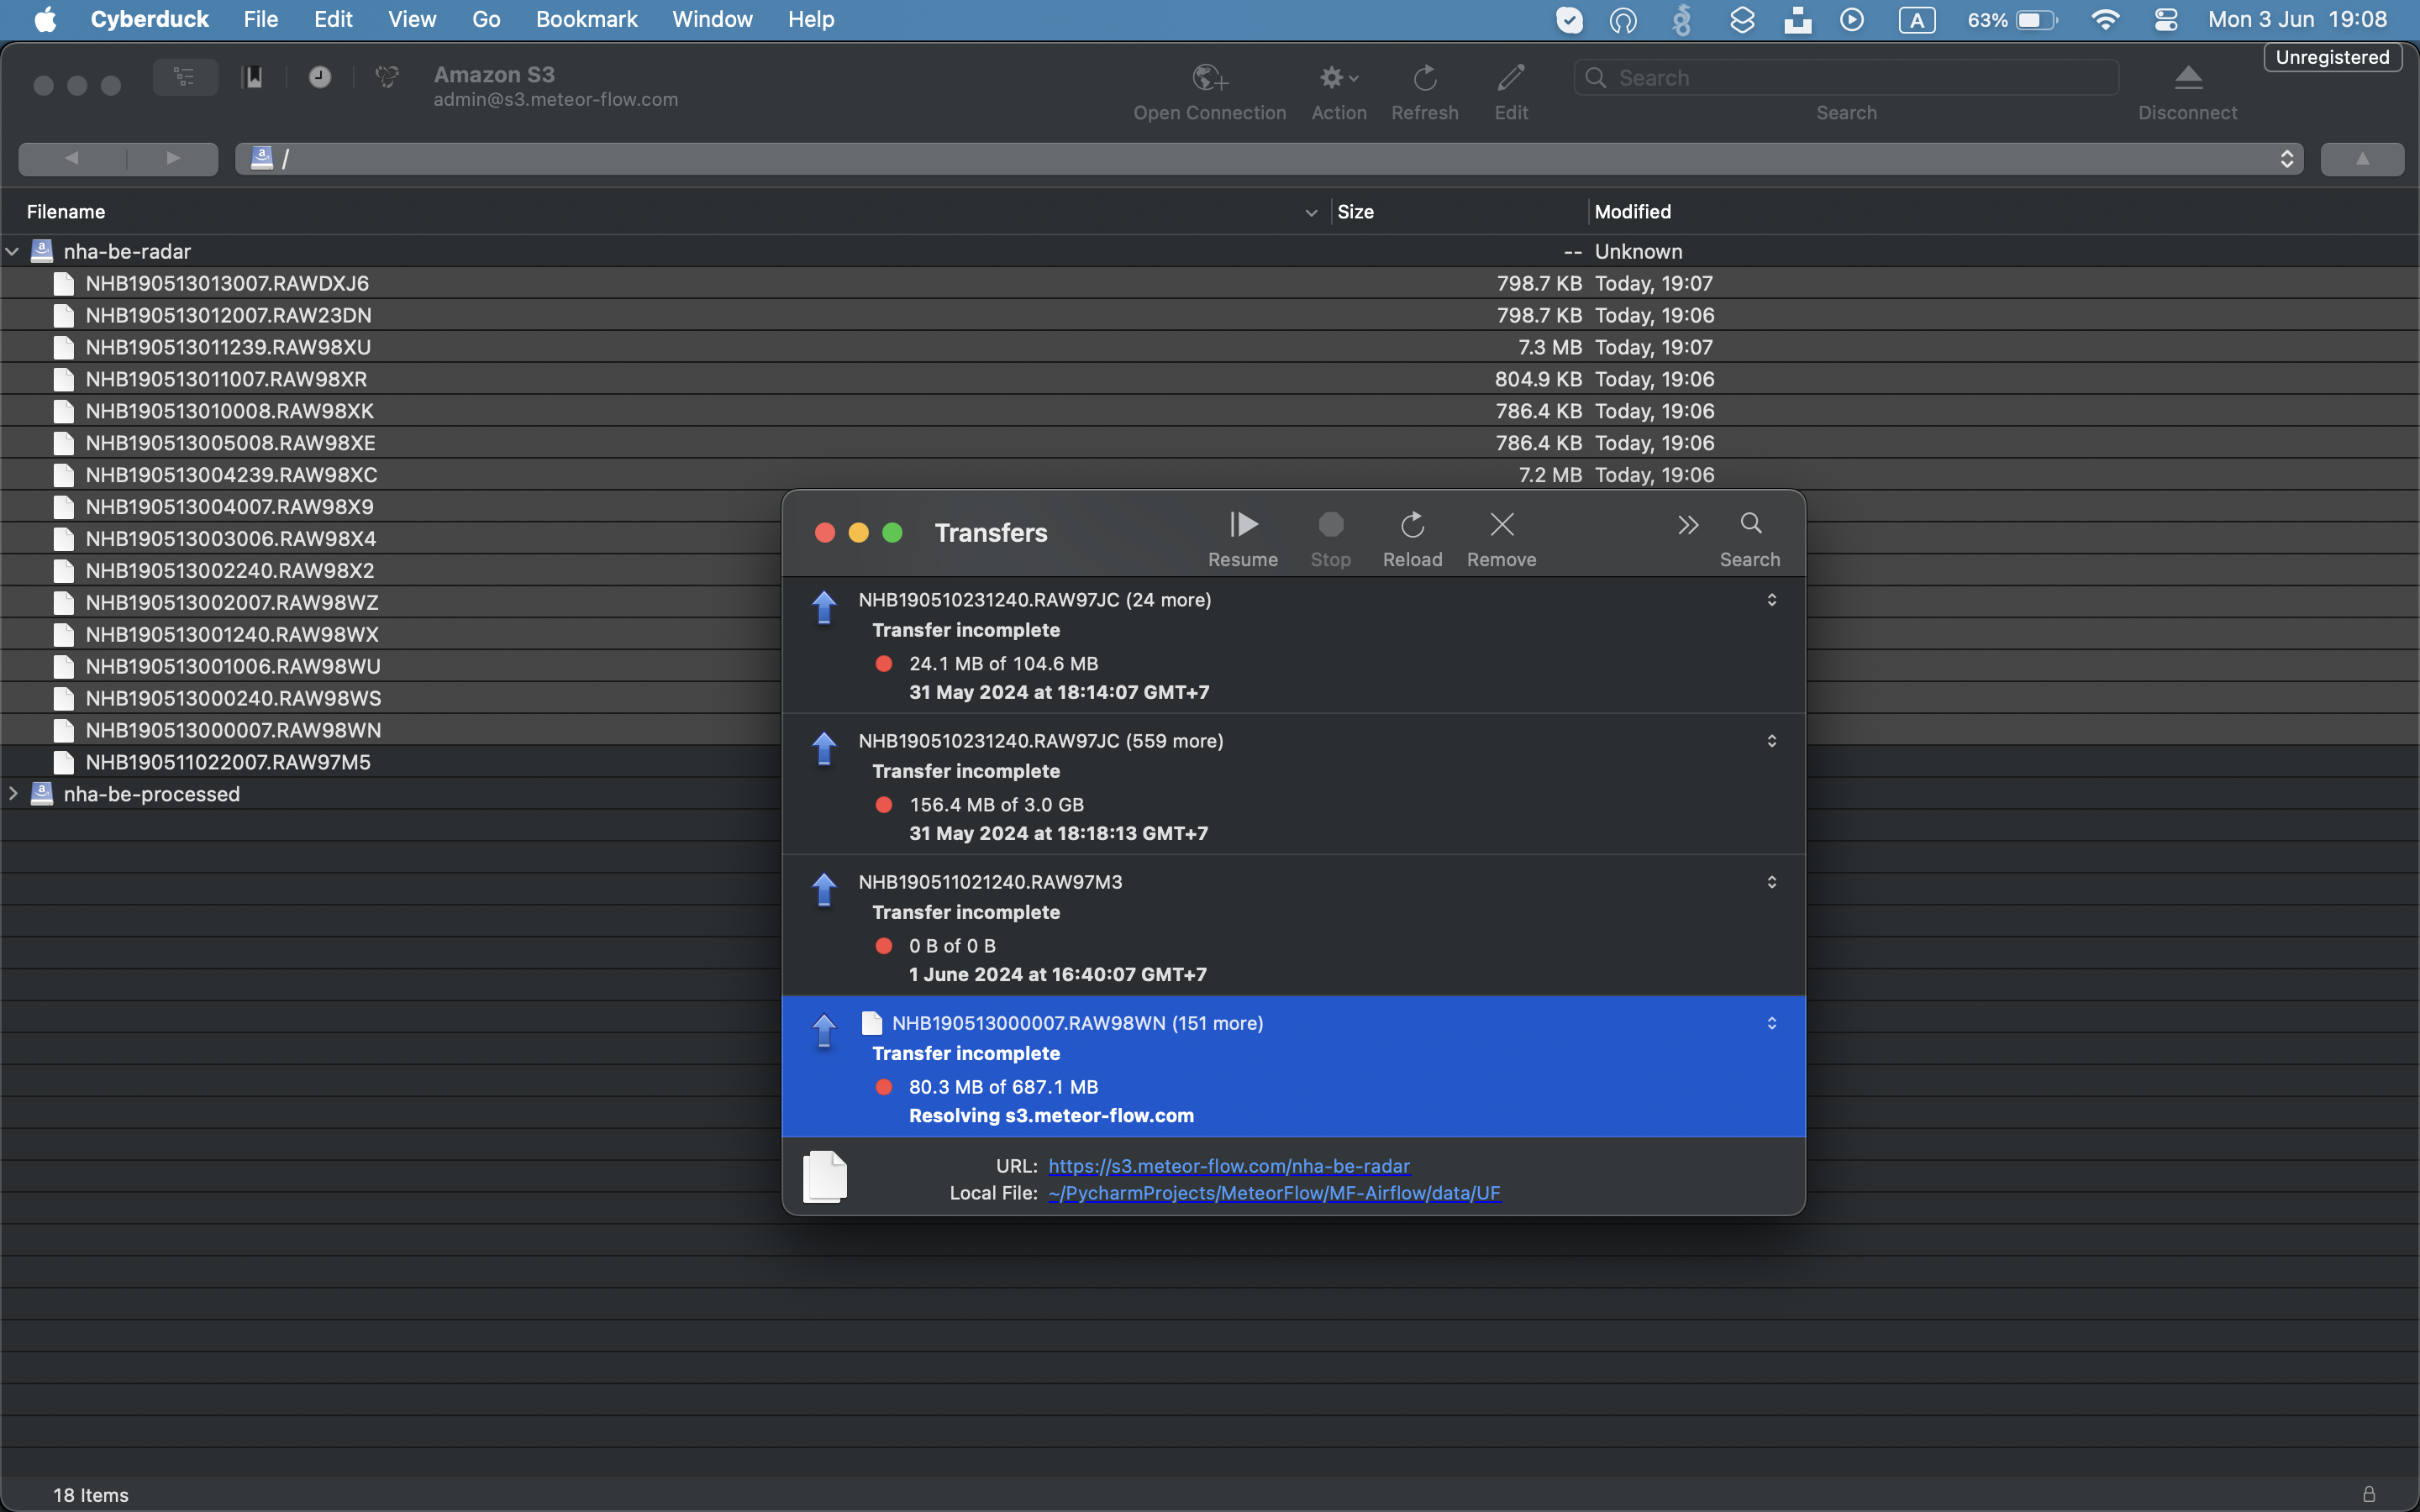
\includegraphics[width=0.8\linewidth]{Images/5-upload-18-files.png}
    \vspace{1cm}
    \caption{Writing files in bulk}
    \label{fig:bulk-write}
\end{figure}

Furthermore, it is imperative to contextualize these empirical findings within
the broader framework of real-world data acquisition scenarios. Notably, the Nha
Be radar generates meteorological data at a frequency of one scan every 10
minutes, thereby necessitating a robust infrastructure capable of seamlessly
handling the influx of data streams from disparate sources. Our empirical
analysis revealed that our system is adept at managing up to 10 concurrent
streams of incoming data, thus affirming its suitability for accommodating the
diverse needs of tenants seeking to integrate with our ecosystem.

Moreover, it is essential to underscore the significance of these findings in
the context of resource optimization and infrastructure scalability. Despite
operating within the constraints of a low-end infrastructure, our system has
demonstrated remarkable efficacy and resilience, underscoring the potential for
leveraging cost-effective hardware solutions to achieve optimal performance
outcomes. This strategic alignment of technological resources with operational
objectives not only enhance the efficiency of our system but also augment its
scalability and adaptability in response to evolving demands and requirements.

In conclusion, the comprehensive testing regimen undertaken by our team has
yielded invaluable insights into the ingestion capabilities of our system,
shedding light on its scalability, resilience, and performance characteristics.
Through meticulous analysis and optimization efforts, we are poised to further
enhance the efficiency and robustness of our infrastructure, thereby laying the
groundwork for a future characterized by unparalleled innovation and excellence
in data management and processing.


\subsection{Processing data}

In pursuit of enhancing the informativeness and query efficiency of our data, as
well as mitigating loading bandwidth concerns, our team has judiciously opted to
undertake preprocessing measures on the provided files. Central to this
preprocessing strategy is the extraction of the "reflectivity" field, a pivotal
attribute within the dataset, which is subsequently stored directly as a NumPy
array. By meticulously orchestrating these preprocessing tasks within the
purview of the Apache Airflow framework, we endeavor to streamline data
manipulation processes while fostering a conducive environment for seamless data
exploration and analysis.

The adoption of Airflow as our orchestration tool necessitated a concerted
effort to optimize and customize the system to suit our specific requirements.
Given the resource-intensive nature of Airflow, the initial deployment and
configuration of a functional cluster posed a formidable challenge for our team.
However, through a collaborative endeavor characterized by heavy optimization
endeavors and meticulous customization efforts, we succeeded in overcoming these
hurdles and achieving a state of operational readiness. This transformative
journey underscored the resilience and adaptability of our team, exemplifying
our unwavering commitment to harnessing cutting-edge technologies for the
betterment of our data management ecosystem.

\begin{figure}[ht]
    \centering
    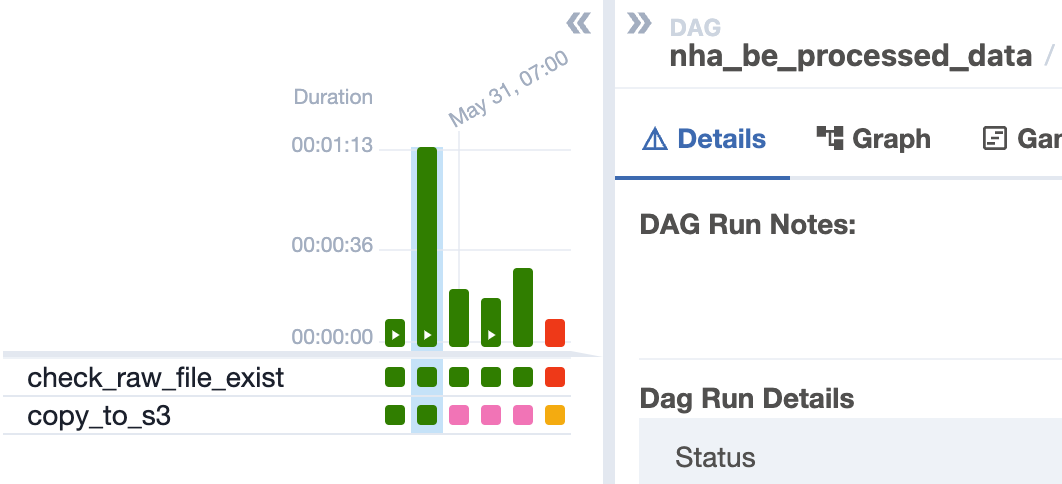
\includegraphics[width=0.8\linewidth]{Images/5-etl-data.png}
    \vspace{1cm}
    \caption{It typically takes about 1.5 minutes to process one file from Nha Be}
    \label{fig:etl-data}
\end{figure}

It is imperative to delineate the tangible outcomes of our optimization
endeavors within the broader context of operational efficiency and system
performance. By fine-tuning the configuration parameters and streamlining the
execution workflow, we have succeeded in substantially reducing the processing
latency associated with data preprocessing tasks. Empirical evidence gleaned
from extensive testing scenarios indicates that our optimized Airflow cluster
can efficiently process a batch of five files, each approximately 30 MB in size,
in less than two minutes. This remarkable feat not only underscores the efficacy
of our optimization strategies but also augurs well for the scalability and
resilience of our data processing pipeline.

Furthermore, it is essential to highlight the transformative impact of our
preprocessing efforts on the overall efficacy of our data management ecosystem.
By distilling the raw data into a concise and structured format, characterized
by the direct storage of pertinent attributes as NumPy arrays, we have
significantly enhanced the accessibility and usability of the dataset.
Researchers and analysts can now leverage these preprocessed datasets to glean
valuable insights and derive meaningful conclusions with unprecedented
efficiency and accuracy, thereby catalyzing transformative advancements across
diverse domains.


\subsection{Concurrently reading data}
Using the PyTorch API that we have implemented, we perform reading data in
multiple processes. This innovative approach not only facilitates seamless
access to our data storage but also serves as a poignant simulation of
real-world scenarios wherein disparate model teams endeavor to interact with our
comprehensive dataset.

Our empirical findings reveal that our servers exhibit commendable resilience
and efficiency in handling the influx of querying threads accessing training
data. Remarkably, our infrastructure demonstrates robust performance even under
moderate load, with the capacity to seamlessly accommodate up to 5 querying
threads without experiencing any detrimental impact on system stability or
performance. This resilience is indicative of the robustness and efficacy of
both the underlying MinIO storage system and our meticulously designed
infrastructure architecture, affirming the soundness of our technological
choices and engineering decisions.

\begin{figure}[ht]
    \centering
    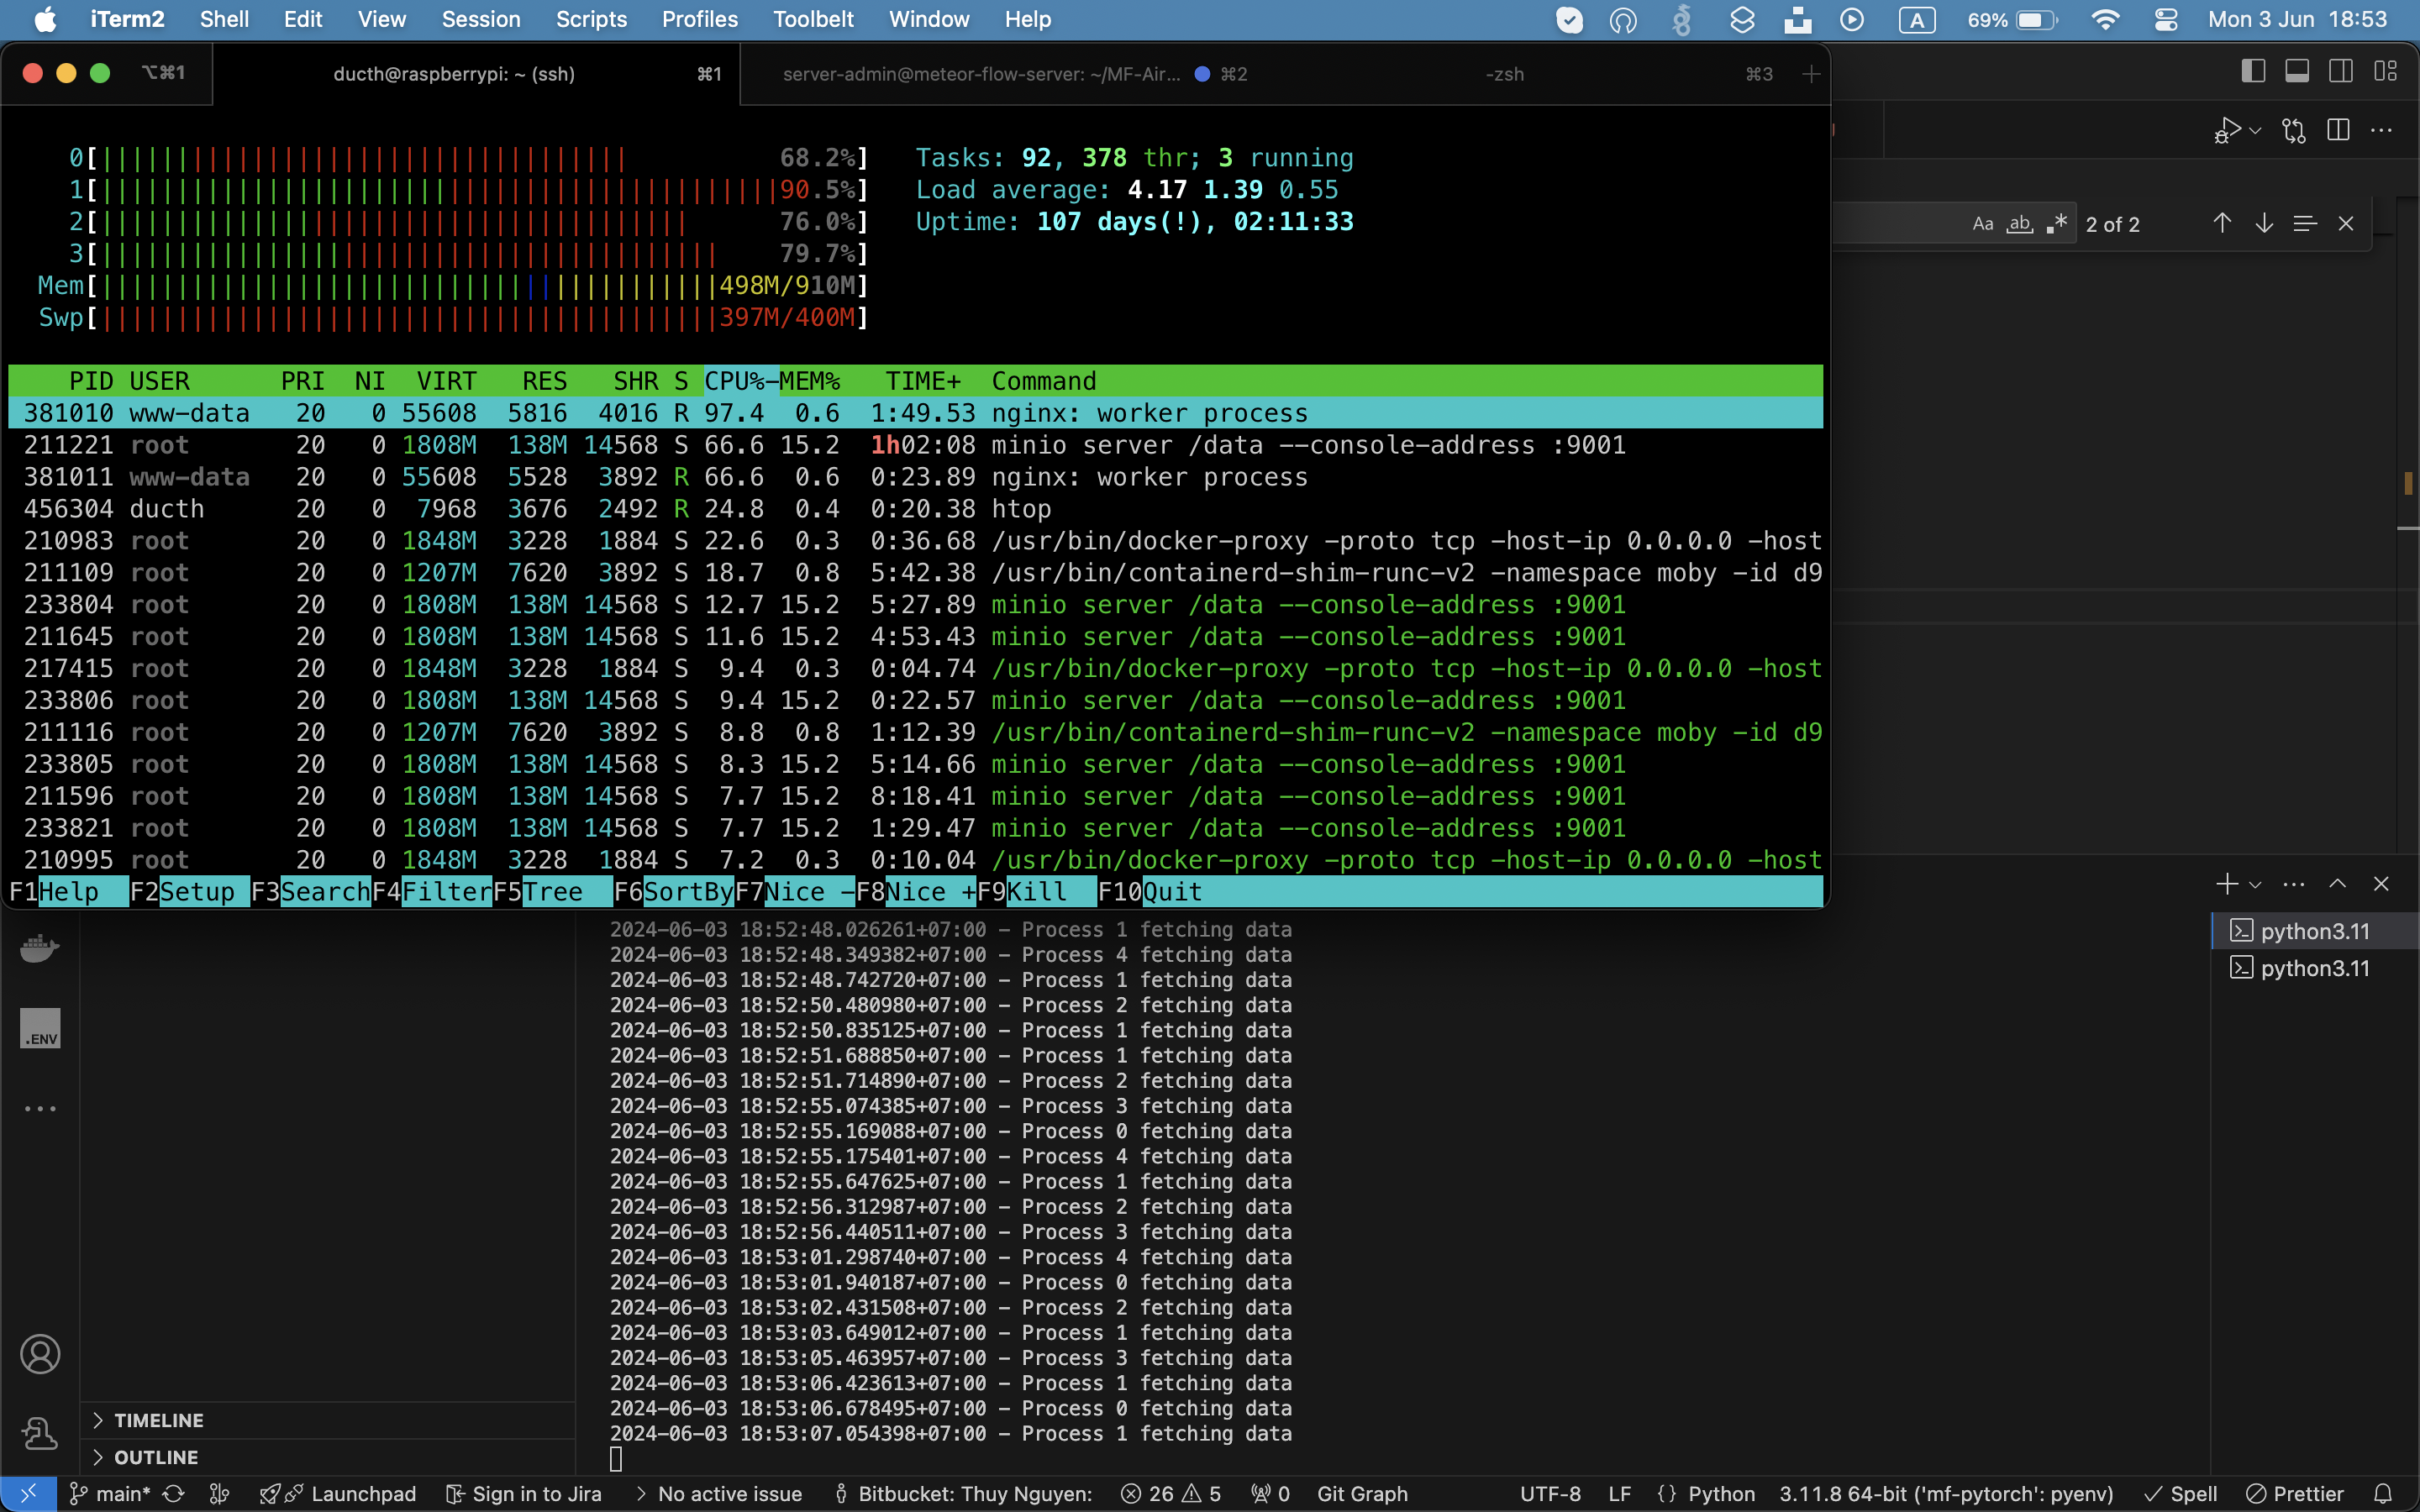
\includegraphics[width=0.8\linewidth]{Images/5-read-5-process-at-once.png}
    \vspace{1cm}
    \caption{Five concurrent thread reading data at the same time}
    \label{fig:concurrent-read}
\end{figure}

It is imperative to contextualize these empirical findings within the broader
framework of model training workflows, wherein the interplay between data
retrieval and model computation is pivotal. From a holistic perspective, the
nominal increase in load time for each batch of data retrieval can be
effectively mitigated by the inherent runtime required for model training
between successive batches. Thus, while there may be a marginal increase in
latency attributable to concurrent querying threads, this impact is mitigated by
the inherent asynchronous nature of model training workflows, thereby ensuring
optimal utilization of computational resources and minimizing potential
bottlenecks.

However, notwithstanding the commendable performance exhibited under current
testing conditions, it is prudent to exercise caution and prudence in managing
concurrent data access requests. Our empirical analysis suggests that while our
infrastructure can robustly handle up to 5 concurrent readers accessing the data
simultaneously, optimal system performance is ensured when the concurrency level
is capped at 3 readers. By imposing this constraint, we can effectively
safeguard the computational resources allocated for write operations, thereby
enhancing system stability and ensuring uninterrupted data ingestion processes.


\section{Further improvement}
In the comprehensive review of our solution, it becomes apparent that while our
system exhibits robust functionality and efficiency, there remain several areas
where additional features or enhancements could be incorporated to further
elevate its efficacy and usability. These missing features represent
opportunities for refinement and optimization, underscoring the iterative nature
of software development and the perpetual quest for excellence.

\subsection{Supports more query types on PyTorch's API}

Presently, within the framework of PyTorch's \texttt{MeteorFlowDataset}, data
retrieval capabilities are confined to querying data within a specified range or
interval of date-time parameters. For instance, users can query data pertaining
to a specific year, such as 2019, or data corresponding to particular dates,
such as the 10th and 11th of June. While this functionality suffices for basic
data retrieval tasks, the burgeoning needs of model teams necessitate the
expansion of query capabilities to encompass more sophisticated and nuanced
requirements.

To address the evolving demands for enhanced data veracity, it is imperative to
augment the existing query models with advanced functionalities that facilitate
comprehensive data exploration and analysis. Among the proposed enhancements is
the integration of support for querying data from combined areas encompassing
two or more radar stations. This strategic augmentation not only facilitates the
seamless integration of disparate data sources but also enhances the granularity
and utility of the information returned.

The implementation of advanced query models, such as querying data from combined
radar areas, represents a pivotal step towards enriching the capabilities of the
\texttt{MeteorFlowDataset} and empowering model teams with unprecedented
insights into meteorological phenomena. By enabling users to aggregate and
analyze data from multiple radar stations simultaneously, we anticipate a
quantum leap in the comprehensiveness and accuracy of the information gleaned
from the dataset.



\subsection{Increase cluster performance}
The current deployment architecture of our system can be characterized as
adequate, albeit with room for improvement. At present, the system is hosted on
two Raspberry Pi 3B+ units, which effectively handle incoming user requests.
However, despite their reliability in meeting current demands, our team has
encountered challenges related to the intricacies of configuring and optimizing
these ARM-based servers. The process of setting up the project entails
meticulous installation of various configurations tailored specifically for
these hardware platforms, often consuming significant time and effort, with
execution times stretching over hours.

While the Raspberry Pi 3B+ units have served as dependable hosts for our
services thus far, there is a palpable sense within our team of the limitations
posed by their performance capabilities. As we strive for continuous improvement
and scalability, it is imperative to explore alternatives that offer greater
computational power and flexibility. Consequently, we envision conducting
extensive research into the feasibility of transitioning to a more robust server
solutions, such as Intel NUCs or basic PCs. By leveraging these
higher-performance hardware platforms, we anticipate a significant enhancement
in our system's capabilities, enabling us to seamlessly accommodate the
anticipated growth in clusters and user base as we integrate with new tenants
and systems.

The envisioned migration to more powerful server hardware represents a strategic
investment in the future scalability and resilience of our infrastructure.
Beyond the immediate benefits of enhanced computational capabilities and
streamlined maintenance workflows, this transition holds the promise of
positioning our system on a trajectory of sustained growth and innovation. With
the agility and versatility afforded by higher-performance server solutions, we
can confidently navigate the evolving landscape of data management and
processing, ensuring seamless integration with emerging technologies and
accommodating the dynamic needs of our expanding user base.

Moreover, the adoption of alternative server hardware opens up avenues for
exploring novel optimization strategies and performance enhancements. By
capitalizing on the inherent strengths of Intel NUCs or basic PCs, we can unlock
new possibilities for fine-tuning our system architecture and streamlining
resource utilization. This strategic alignment of hardware capabilities with
operational objectives underscores our commitment to continuous improvement and
innovation, fostering a culture of excellence and resilience within our
organization.